\chapter{Design Intuition for Energy Harvesting Systems}
\label{chap:intuition}

\section{Is Energy Harvesting Worth It?}

\placefigure{fig:intuition:eh_worth_it}

\section{Defining the Application Space}
The designed purpose of a wireless sensor is generally a simple one: measure some phenomena, optionally perform some filtering or calculation on that measurement, and transmit the results. 
This has been the prevailing archetype of research and industrial sensing since the inception of wireless sensor networks. 
The acceptable reliability, and reporting frequency is highly dependent on application requirements. Many safety critical or industrial applications require high reliability and frequent and immediate sensing and reporting. Conversely, an amount of unreliability, incomplete data, or reporting delay is acceptable in some citizen science sensing applications, where any data is better than no data.

This section seeks to better explore the design space of wireless sensors, especially with respect to how requirements on the kind of data being reported, the reporting frequency, and reliability, affect the requirements on the sensor power supply design. 

\subsection{Data type}

\subsubsection{Counting}

\subsubsection{Measurement}

\subsection{Reporting Frequency}

\subsubsection{Periodic}

\subsubsection{Reactive}

\section{A Taxonomy of Wireless Sensor Power Supply Architectures}
\label{sec:intuition_related}

Prior work regarding energy harvesting sensor systems can be broadly
divided into two categories: those which make use of intermittent computing
techniques and those which do not.
Intermittent systems often exist in a regime of unreliable and ultra low harvester power, where
operation and uptime are not guaranteed. As such, they often lose power and
reboot while intermittently working through a sensing task.
A wealth of work has been devoted to
making these systems usable and reliable.
Other energy harvesting systems, especially those deployed outside, have access
to significantly more harvestable energy and are able to store more of this energy
for later use, so they
do not use intermittent computing techniques to complete their workloads.
\subsection{Intermittent Sensors}
\label{sec:related:intermittent}

Energy harvesting systems that rely
exclusively on repeatedly buffering small amounts of energy to
operate are commonly referred to as intermittent systems.
Many choose to employ
capacitors as an energy buffer due to their theoretically infinite lifetime,
but are limited to small energy capacities, and are only as reliable and
lively as their source of harvested energy.
In situations of energy drought, 
these platforms often deplete their 
small energy stores, and lacking energy,
they power off and lose
state, potentially in the middle of an important operation or for an extended
period of time.
\\

\vspace{-6pt}
\noindent
\textbf{One-shot Intermittency.}
The Gecko and Monjolo platforms ignore the difficulties associated with
completing longer workloads and instead allocate
just enough capacitance to turn on and perform a simple task. Sometimes, the
rate of harvesting is the sensor itself~\cite{campbellEnergy14,
yervaGrafting12, debruin2013monjolo}.  However, this approach can require
tedious and non-standard optimization of the cold start process and is severely
limited in its simplicity. Performing any sensing or computing outside of the
hardware's intended use case is often not possible,
and it is difficult to distinguish sensor failure from a lack of energy.
\\

\vspace{-6pt}
\noindent
\textbf{Checkpointing.}
Other work in this space attempts to cope with
intermittency
by developing tools and
programming language primitives that allow %can perform
complex and energy intensive tasks to execute despite limited energy storage.
Intermittent-aware programming
models and compilers were developed to enable checkpointing and progress latching over
workloads that may require more energy than can be stored or harvested in a
reasonable time~\cite{lucia2015simpler, ransford2012mementos, hesterTimely17}. New debugging tools
spanning both the hardware and software domains
measure the energy required for specific code operations
and restore energy state during code breakpoints~\cite{colin2016energy}.
\\

\vspace{-6pt}
\noindent
\textbf{Hardware Hysteresis Management.}
In addition to intermittent software techniques,
hardware platforms have been developed to
increase availability and responsiveness through the fine-grained management
of capacitor charging hysteresis.
For these systems,
it is often assumed that the upper hysteresis threshold, the point at which a
charging device turns on, is the voltage at which a capacitor is full, and the
lower threshold, the point at which the system turns off or sleeps, is the minimum
operating voltage of components in a system.
Smaller capacitors can charge to an upper
threshold and turn on faster, but store less energy.  Hysteresis management
techniques attempt to combine different sized capacitors to
minimize charging time while also maximizing available energy.

The Flicker
platform employs federated
energy storage in which each peripheral has its own storage tuned to the task
it is expected to perform~\cite{hesterTragedy15,hesterFlicker17}. This has the
effect of allowing various components to charge their storage faster, as well
as isolating power failure to independent components.  The Capybara platform is
similar, but provides even more flexibility by dynamically resizing its banked
capacitor store to match the energy required by a task
~\cite{colinReconfigurable18}. This leads to the lowest possible cold start and
capacitor recharge times to support a given
operation.

We believe the assumption that operation should be coupled to full-swing hysteresis
is not valid
for many systems. Capybara does explore the possibility of setting an upper
threshold to less than the maximum voltage and using an adjustable bottom
threshold instead of dynamically resizing their capacitor store.
However, they disregard these options due to high voltage comparator
power and long cold start times, respectively.
While these decisions make sense in this context, the importance they place on cold start optimization
is specific to their design. Capybara's power supply has a significant
"power overhead of the power system" that limits the effectiveness of
sleeping. Due to this, they opt to fully discharge their storage on every
operation and optimize cold start.  In practice, if a system has the ability to
enter a low power sleep mode or power off, it can
avoid cold start and control its energy usage by willfully entering these
states. With this operating principle, the benefits of hardware hysteresis management
are limited to reducing cold start time and are workload independent.

These complex software and hardware solutions, while increasing usability and reliability, do not address the singular problem for capacitor-based energy
harvesting systems: in the face of plentiful harvestable energy, they are not
able to store the energy for later use (in times of energy drought).
As a result, they must
micro-optimize the little energy they have.  In many applications, if these
systems had sufficient capacity, they could instead adjust sensing rate and
workloads over periods of days or weeks.  We show that the energy captured
by these systems and their subsequent availability
could be substantially improved by using larger energy buffers.
\subsection{Non-intermittent Sensors}
\label{sec:related:nonintermittent}
Non-intermittent energy harvesting sensors
have largely existed in environments with plentiful harvestable energy
and have been designed with sufficient capacity to capture this energy. Some
devices have also embraced backup primary-cells to further ensure
reliable operation.  \\

\vspace{-6pt}
\noindent
\textbf{Rechargeable Batteries.}
Most examples of such devices are deployed outdoors.
For these systems, the obvious choice is to use secondary-cells, as they can
better capture a significant portion of copious solar energy
~\cite{jiang2005perpetual, kansal2007power, corke2007long, lin2005heliomote, adkins2018signpost}.
Most notable of this group is Prometheus,
which utilizes a supercapacitor as a short term energy store, and when full,
charges a backup rechargeable lithium battery~\cite{jiang2005perpetual}. At
the time of its design, lithium cells offered highly limited recharge cycles,
and by utilizing a supercapacitor, much of this
charge-discharge volatility was masked from the secondary-cell, extending its lifetime.
Rechargeable batteries have also been applied to indoor sensing.
The EnHANTs sensor uses an intentionally oversized NiMH
battery, with plans to eventually use a thin-film battery~\cite{margolies2015energy}.
While the choice to use batteries allows for more energy capacity,
NiMH and thin film chemistries offer poor
energy density and lower cycle life compared to lithium
based chemistries. DoubleDip and other sensors~\cite{martin2012doubledip,raisigel2010autonomous} use a
lithium-manganese battery.  DoubleDip notes that supercapacitors offer
lower energy density and higher leakage when compared to batteries, but admits
that the lithium-manganese chemistry suffers from low maximum output currents
and a limited number of charge-discharge cycles.
While the limitations of past batteries have slowed their adoption in
low energy harvesting scenarios, we claim that recent developments in battery
technology will enable higher capacity energy storage without these trade offs.
\\

\vspace{-6pt}
\noindent
\textbf{Backup Energy Store.}
Regardless of which energy store is used, energy harvesting systems will
experience some degree of intermittency. We advocate that a non-rechargeable
backup energy store can be utilized to mask this intermittency, cold
start electrical components, and provide consistent, reliable, and lively operation.
The only system we find that employs a non-rechargeable
backup is the Pressac line of capacitor-based energy harvesting sensors which
use battery backup to obtain an estimated 10 years of continuous operation
\cite{pressac}.  This work suggests that these sensors could significantly
increase their lifetime by using a larger secondary energy store.
There has been little
exploration on the benefits of this hybrid design and the use of
primary-cells to avoid intermittency, cold start harvesting circuits,
and provide baseline reliability.


\section{A Framework for Energy Harvesting Power Supply Design}
\label{sec:framework}
We seek to illustrate the design space for energy harvesting sensors in two
ways. The first defines an energy harvesting sensor framework to examine
when designs are feasible and when they require intermittent techniques to make meaningful forward progress.
The second examines dynamic income energy and device behavior through numerical
modeling and simulation.  The framework is based on three key metrics:
harvested energy income, workload, and capacity.
\placefigure{fig:framework}

\subsection{Sensor Regimes}
\label{sec:framework:regime}
The framework splits the design space into four main regimes: always on,
infeasible, checkpointing required, and no intermittent techniques required.
These regimes and their constraints are illustrated in \cref{fig:framework},
and explained in more detail below. \\

\vspace{-6pt}
\noindent
\textbf{Always On.} If the energy harvester supplies a sensor with
more power than the max power it will ever draw, then the device needs
no energy buffer capacity to remain operational. If this is not the case,
then a sensor must have some ability to buffer energy to use when its
operating power exceeds than the harvester input power.
\\

\vspace{-6pt}
\noindent
\textbf{Infeasible.} If the energy harvester supplies less power than
the system leakage, the energy buffer will never
charge. If the energy buffer capacity is less than the
energy required to perform a workload's largest atomic operation, with energy harvested
during the operation itself, then that operation will not have enough energy to
complete.  Neither of these designs will make forward progress and are
therefore infeasible.
Common atomic operations on energy harvesting sensors include sampling a sensor,
sending a radio packet, booting the processor, and performing a checkpoint.
\\

\vspace{-6pt}
\noindent
\textbf{Checkpointing Required.} If the energy buffer can
hold enough energy to perform atomic operations, but
not enough to complete
workloads composed of multiple, chained
atomic operations (such as sampling a sensor and then sending a radio packet), then
a mechanism for saving state and continuing progress on the next reboot
must be employed.
\\

\vspace{-6pt}
\noindent
\textbf{No Intermittent Techniques.} A sensor that has enough harvester
potential and energy capacity to complete a workload's longest non-atomic
operation can operate without checkpointing. Such systems also benefit as
energy devoted to checkpointing can be used for a workload instead.
\\

\vspace{-6pt}
\noindent
\textbf{Hysteresis Management.}
Finally, if a sensor's deep sleep power draw %willfully powers down
is a substantial fraction of the harvester power, as
is the case with Capybara~\cite{colinReconfigurable18}, then it is
beneficial to continue operating until the energy
buffer is depleted, power off, and recharge quickly
rather than stop early and recharge slowly.
Under this scenario, hysteresis management techniques,
such as reconfigurable capacity and federated energy can increase sensor
performance as discussed in \cref{sec:related}.
The utility of hysteresis management is diminished
when the ratio of harvester power to deep sleep power increases.
For sensors that can willfully power off or sleep,
operating thresholds can be controlled, disentangling
capacity and charging hysteresis.
Their deep
sleep power is equal to leakage, and such techniques
will not improve recharge times.

For all systems, these techniques can decrease cold start time
by reducing the capacity that must be charged
to achieve cold start.

This is more beneficial for systems that cold start frequently and
have a higher energy capacity, however,
a higher-capacity energy store also has a lower probability of
needing to cold start. Therefore the benefits of hysteresis management for
cold start with respect to storage capacity are in conflict with their necessity,
and we do not attempt to quantify these subtle nuances in \cref{fig:framework}.

\subsection{Framework Limitations}
\label{sec:framework:limitations}
This framework makes a couple simplifying assumptions that prevent it from
fully capturing the richness of the design space.\\

\vspace{-6pt}
\noindent
\textbf{Backup Energy Store.}
This framework does not consider the impact of a backup energy store.
%that is pre-charged before the sensor begins operation.
%The simplest way
%to view
A backup energy store can be viewed as the ability to inject additional energy
to the system at arbitrary times,
%move the system
%outside of the regime of requiring checkpoints for very energy intensive operations, or
eliminating the need for checkpointing when there is very low
harvesting potential.

A backup energy store could also contribute in more subtle ways. It could
allow a system to avoid the energy and complexity of checkpointing by
providing just enough energy for a deep sleep mode with state retention rather
than a full power down when the system depletes its stored energy. It could also
cold start energy buffer charging to eliminate the need for reconfigurable
power supplies, or to increase the efficiency of
the energy harvesting front-end at low voltages.
Finally, in periods of long energy drought, the backup energy store could increase
sensor availability.

While the use of a backup energy store
does constrain the sensor to a finite lifetime,
%especially since current technology favors non-rechargeable, primary-cells as
%backup energy stores,
energy harvesting can substantially extend these lifetimes under certain harvesting
conditions.\\
%We explore the lifetime of energy harvesting
%designs with backup energy stores in \cref{sec:primary}.

\vspace{-6pt}
\noindent
\textbf{Constant Harvester Power.}
The framework assumes an energy harvester will supply a constant energy
income, when in reality income is often highly variable. In practice, a sensor
platform both defines the regions of the plot, and occupies a
vertical line which represents the energy storage capacity of the sensor
combined with the range of harvester input powers it might experience. We expect
this line will span multiple regions for most sensors.

However, by ignoring variability, the plot also fails to illustrate key benefits
of capacity under varying energy incomes and workloads. Intuitively,
higher energy buffer capacity can store energy in times of excess and supply
that energy in times of drought. This balancing out of energy income
effectively raises the minimum power supplied by the energy harvester.
Because the extent of this impact is completely dependent on the variability
of the energy income and workload of the sensor, we also develop a numerical simulation to
quantify the impact of capacity
on key metrics including energy utilization, availability and reactivity.

\section{Application feasibility}

\section{An Intuitive Case for Capacity}

\begin{definetable}{tab:related}
  \scriptsize
  \begin{threeparttable}
  \centering
  \begin{tabular}{l | c c| c c| c}
      \multirow{2}{*}{Platform} & \multicolumn{2}{c|}{Successful Events\,(\%)}  & \multicolumn{2}{c|}{\parbox{2.5cm}{\centering Long-Running\\Time to Completion Ratio}} & \multirow{2}{*}{Lifetime\,(yrs)}\\
                              & Periodic     & Reactive                     & Average & 95th Percentile & \\
    \hline
    Telos \cite{polastre2005telos}                      & 100   & 100   & 1     & 1     & 8.55\\
    Hamilton \cite{kim2018system}                & 100   & 100   & 1     & 1     & 6.75\\
    BLEES \cite{adkins2015michigan}                     & 100   & 100   & 1     & 1     & 1.11\\
    Gecko \cite{yervaGrafting12}                 & 39.5  & 64.9  & 387   & 981   & $\infty$\,\tnote{g} \\
    Capybara~\cite{colinReconfigurable18}\,\tnote{a}    & 46.3  & 72.8  & 37.6  & 1     & $\infty$\,\tnote{g}\\
    Capybara~\cite{colinReconfigurable18}\,\tnote{b}    & 41.1  & 67.1  & 2730  & 8900 & $\infty$\,\tnote{g}\\
    Flicker \cite{hesterFlicker17}                      & 39.3  & 64.2  & 1307  & 5670 & $\infty$\,\tnote{g}\\
    EnHANTs \cite{margolies2015energy}                  & 79.4  & 96.0  & 1     & 1     & \textemdash\,\tnote{h}\\
    DoubleDip \cite{martin2012doubledip}                & 77.9  & 66.5  & 1     & 1     & \textemdash\,\tnote{h}\\
    \cite{raisigel2010autonomous}                       & 78.4  & 66.9  & 1     & 1     & \textemdash\,\tnote{h}\\
    \textbf{\name}\,\tnote{c}                           & 81.2  & 98.3  & 1     & 1     & \textemdash\,\tnote{i}\\
    \textbf{\name}\,\tnote{d}                           & 100   & 100   & 1     & 1     &  35.8\\
    \textbf{\name}\,\tnote{e}                           & 100   & 100   & 1     & 1     &  30.2\\
    \textbf{\name}\,\tnote{f}                           & 100   & 100   & 1     & 1     &  6.27\\
  \end{tabular}
    \begin{tablenotes}[para]
      \item[a] With capacitors: 400\,\si{\micro\farad} ceramic + 330\,\si{\micro\farad} tantalum + 67.5\,mF supercapacitor.
      \item[b] With capacitors: 300\,\si{\micro\farad} ceramic + 1100\,\si{\micro\farad} tantalum + 7.5\,mF supercapacitor.
      \item[c] No primary-cell.
      \item[d] AA primary-cells like Telos.
      \item[e] CR123A primary-cell like Hamilton.
      \item[f] CR2032 like BLEES.
      \item[g] Lifetimes are theoretically infinite for capacitor-based systems.
      \item[h] Not enough information to predict cycling failure time for theses systems.
      \item[i] Expect cycling failure in 20-50 years, but do not attempt to estimate.
    \end{tablenotes}
  \end{threeparttable}
  \caption{
  \normalfont
      Modeled performance of energy harvesting systems.
    For each  platform considered, we model the performance of its energy storage
    architecture. Periodic workload and lifetime estimates are based on a 10\,s
    period, and the reactive workload is scaled to
    generate a maximum of 2000 events per hour (3.4\,s average daily period). Generally,
    intermittent systems have significantly worse availability and responsiveness compared to
    battery-only systems and systems that use a secondary-cell. Battery-only
    systems achieve perfect operation, but have finite, sub-decade lifetimes.
    }
\end{definetable}

\begin{definefigure}{fig:framework}
  \centering
  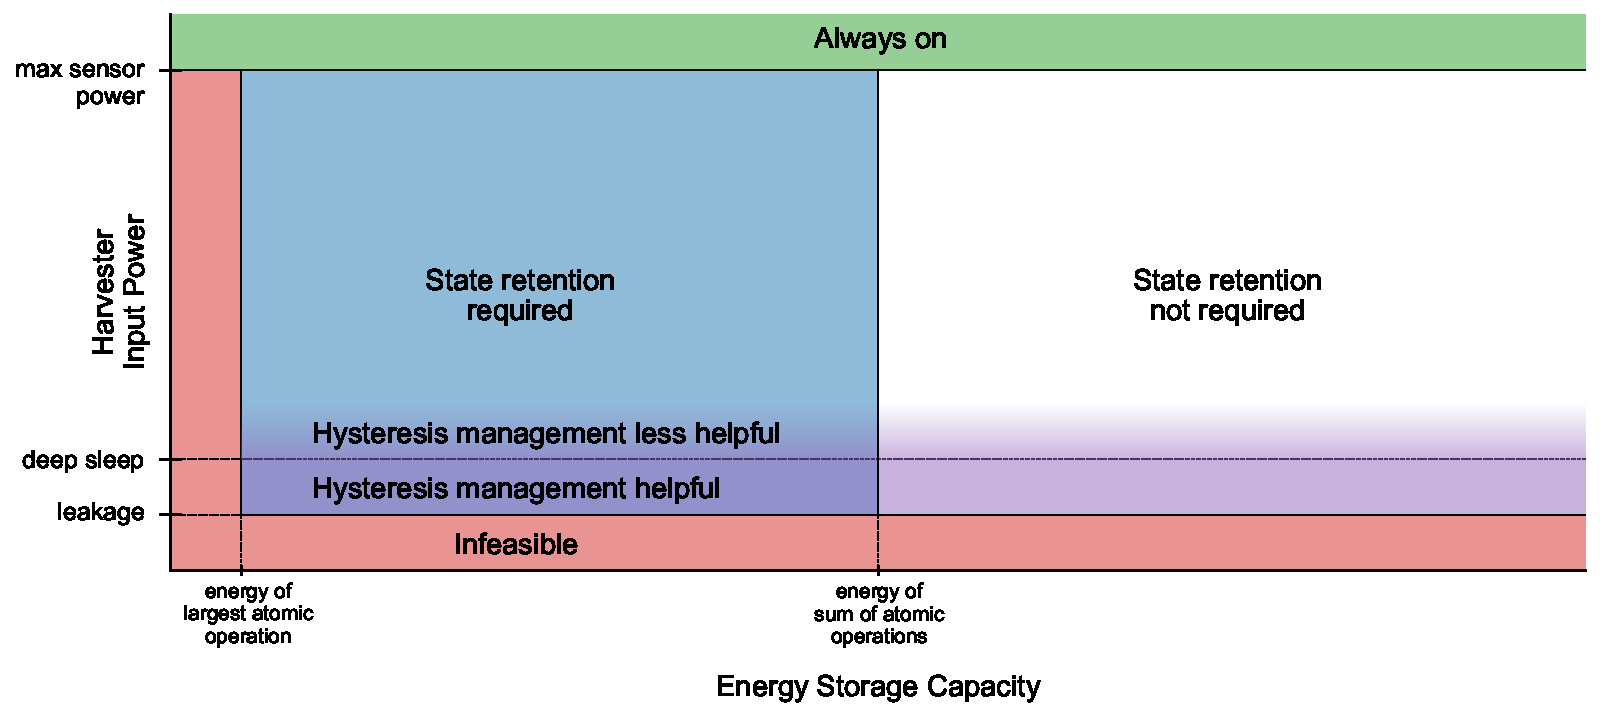
\includegraphics[width=\columnwidth]{figs/capacity/harvesting_framework/framework}
  \caption{
  %Energy harvesting
  %sensors have different capabilities and requirements
  \normalfont Design space for energy harvesting sensors based on their energy
  income (which we assume is constant for this analysis), energy storage capacity, and workload.
  Workload is represented by the largest atomic/non-atomic operations supported
  by a design, as well as the deep sleep and leakage power.  The plot breaks
  into four regions: \textbf{1)} always
  on or effectively powered, \textbf{2)} Infeasible due to lack of energy storage or
  leakage higher than harvesting rate \textbf{3)} Feasible but requires checkpointing
  to make forward progress, and \textbf{4)} Enough energy storage to not require
  or benefit from checkpointing. Additionally, sensors which have high
  power when they enter deep sleep before depleting their
  energy buffer may benefit from hysteresis management techniques.
  This benefit diminishes with lower sleep currents and higher harvesting potential.
  %With increased capacity, sensors can avoid the complexity of intermittent
  %programming techniques and specialized, reconfigurable power supplies in addition
  %to the other benefits of increased capacity discussed
  %in \cref{sec:store}.
  }
\end{definefigure}


\begin{definefigure}{fig:intuition:eh_worth_it}
  \centering
  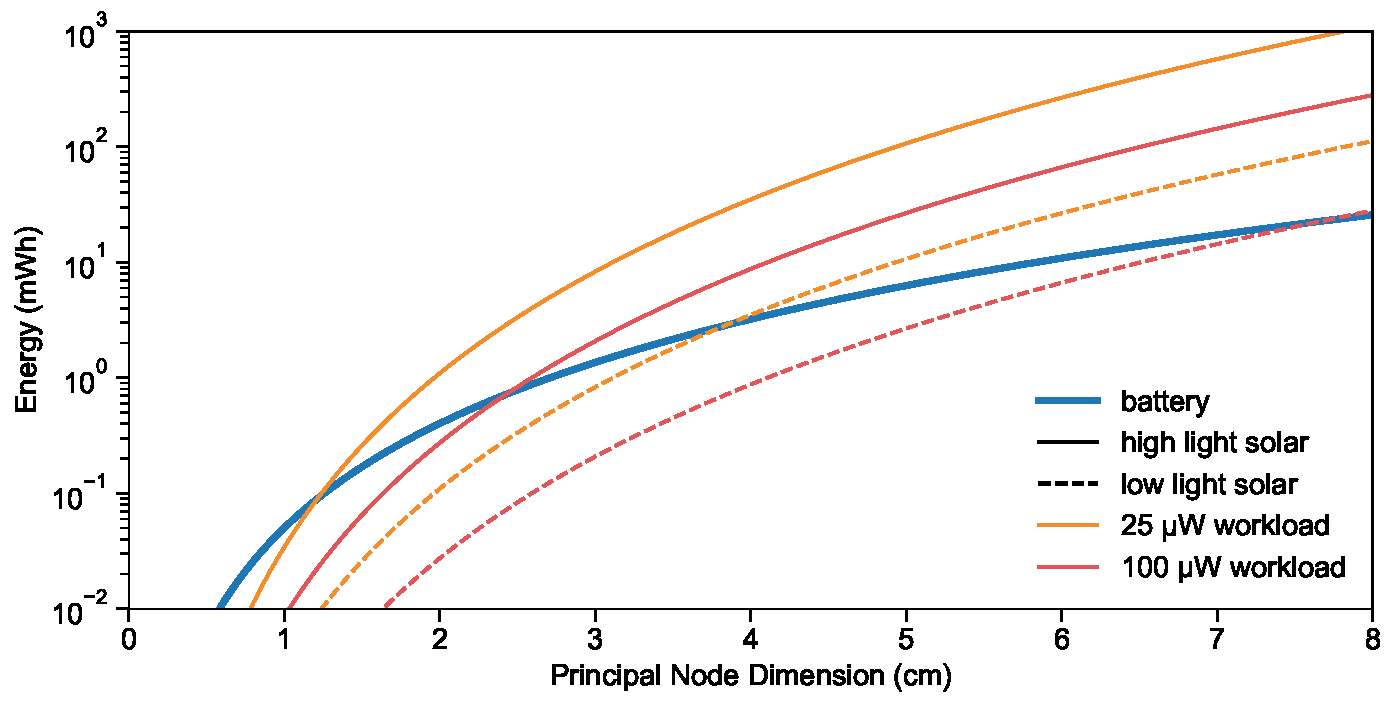
\includegraphics[width=\columnwidth]{figs/is_eh_worth_it.pdf}
  \caption{
  blah
  }
\end{definefigure}